\chapter{Architecture of GRAPHINIUS}
\label{ch:graphinius_architecture}

\begin{figure}[ht]
	% \centering
	\hspace*{-0.5cm}
	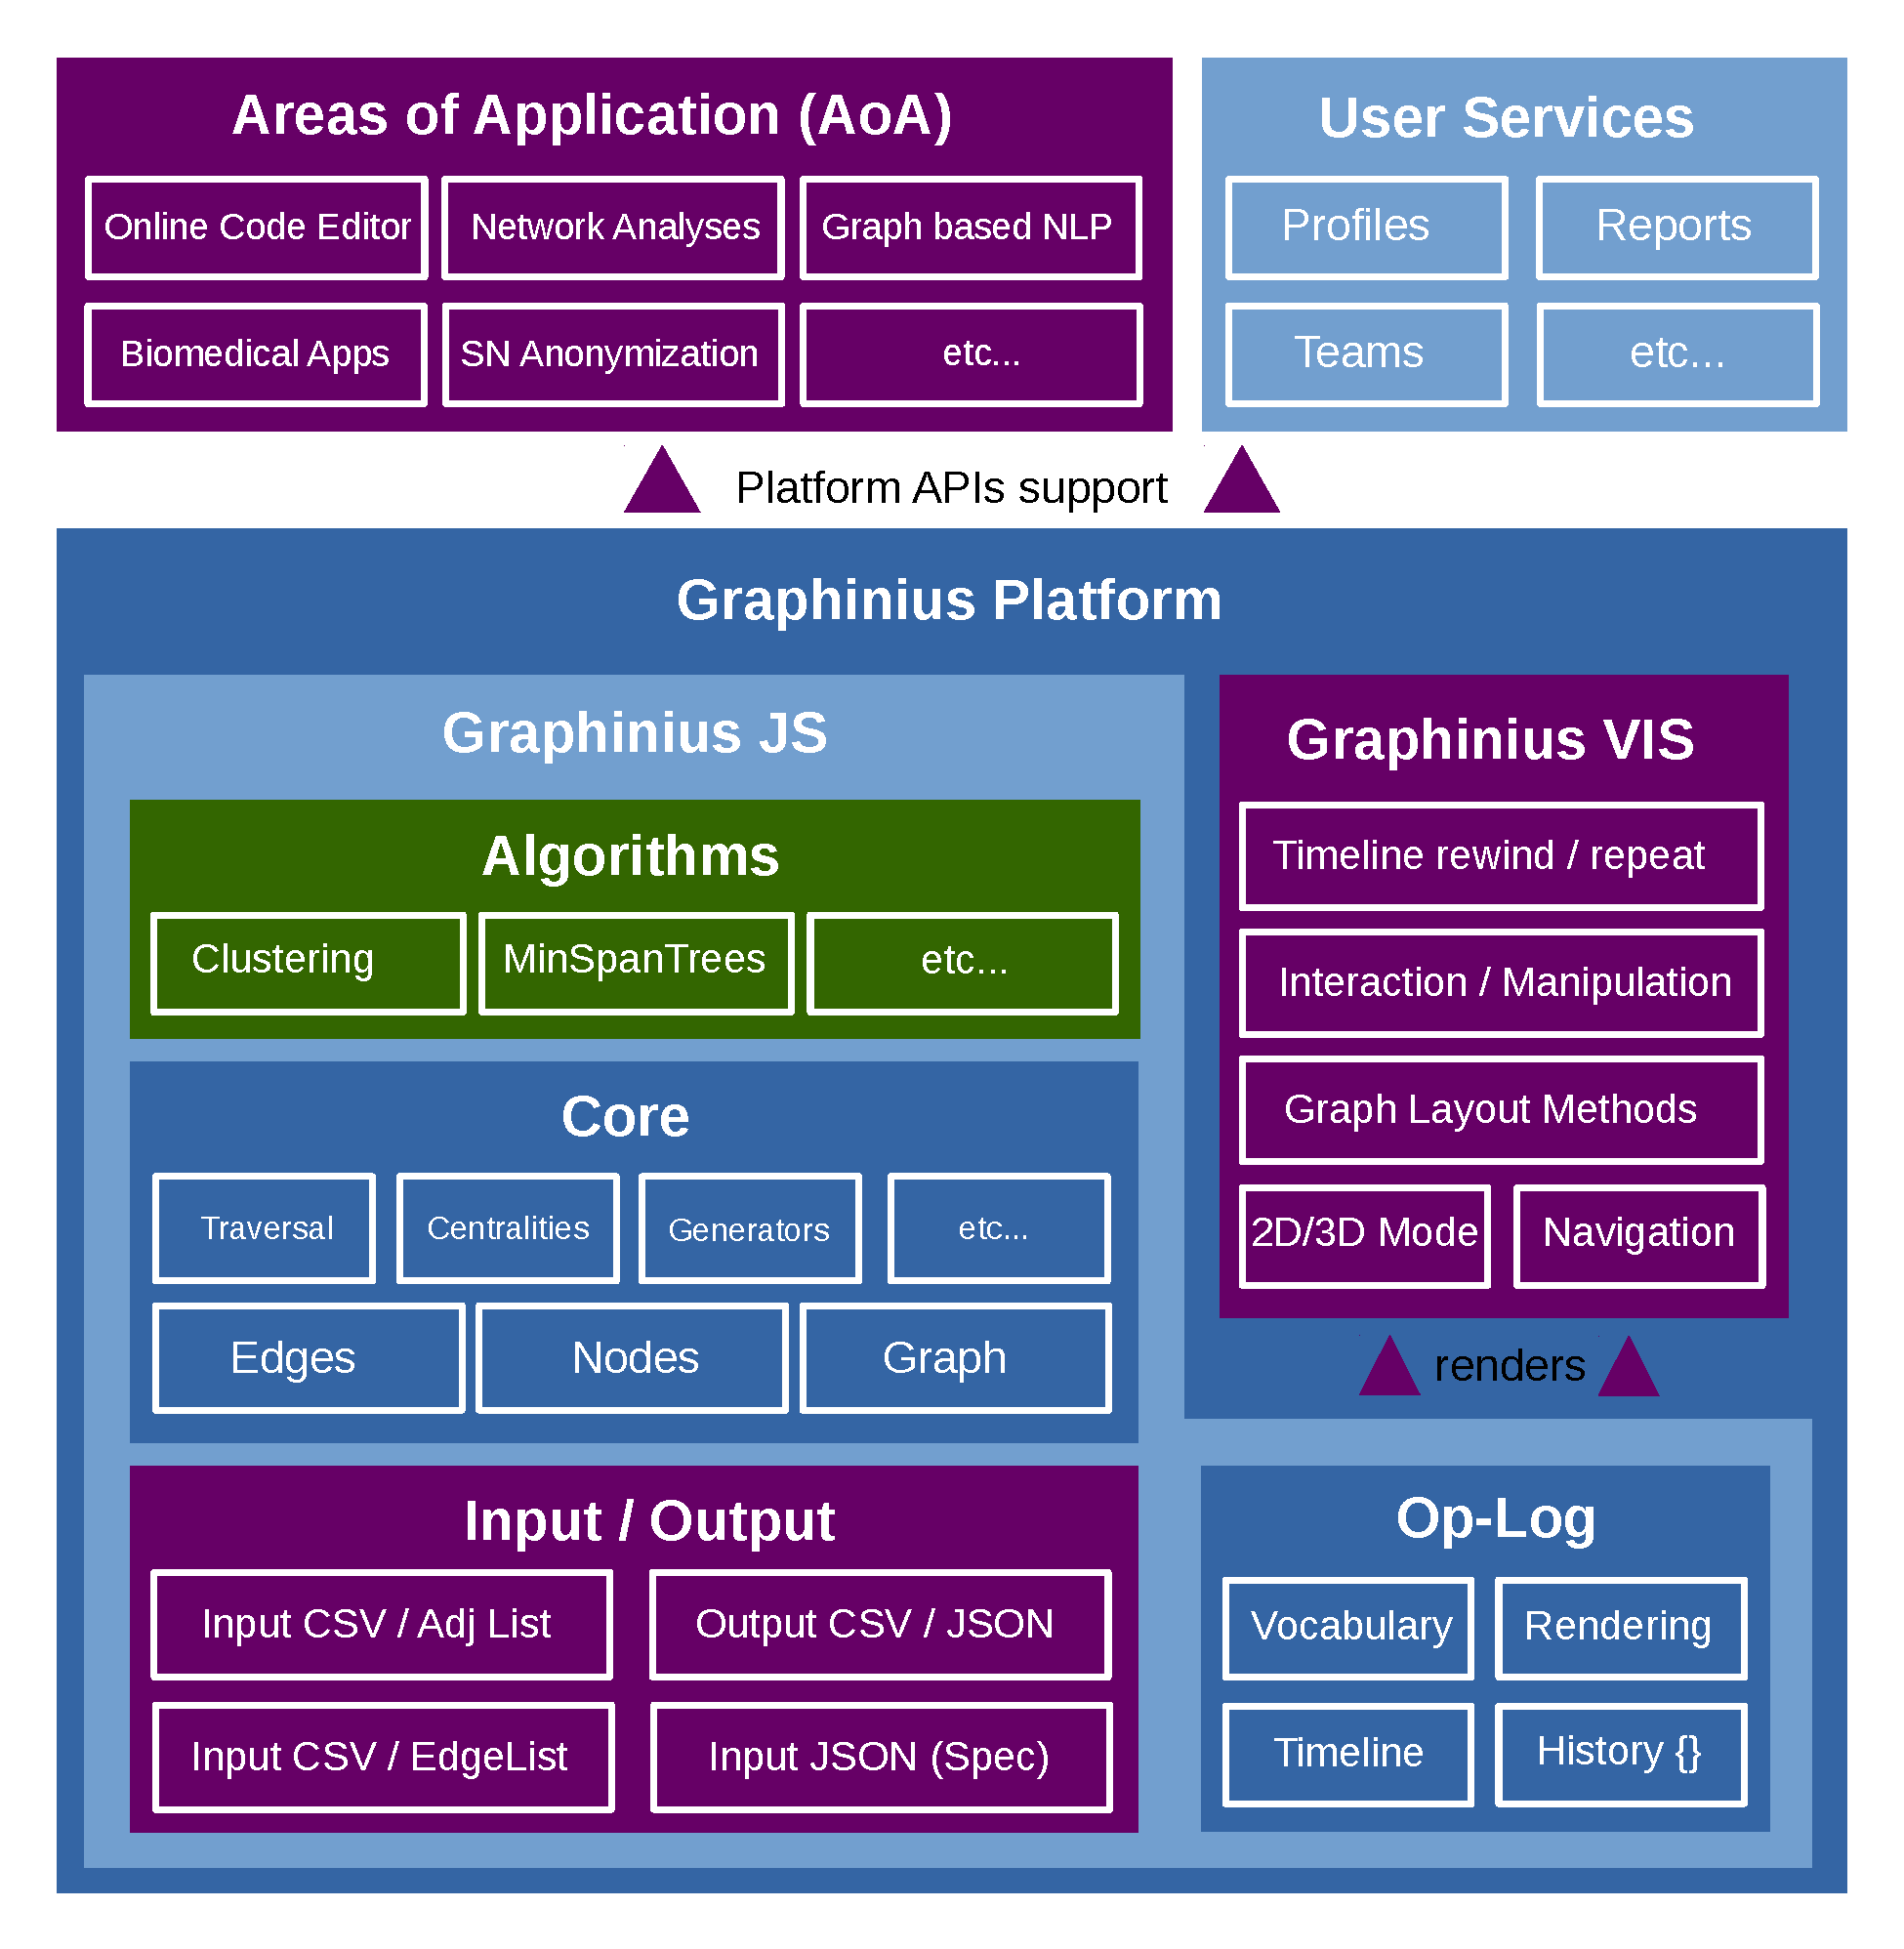
\includegraphics[width=1.1\textwidth]{figures/Graphinius_Architecture_pdf}
	\caption{Graphinius platform architecture overview}
	\label{fig_graphinius_architecture}
\end{figure}



\section{Graphinius Base}
\label{sect:graphinius_base}

As the name suggests, the Base offers all the functionality necessary to develop graph-based applications on top of it, including basic graph-computations and algorithms as well as visualization. It is therefore logically composed of those two modules, Graphinius JS and Graphinius VIS as well as a mechanism of communication between those two.
	

\section{Graphinius JS}
\label{sect:graphinius_js}

	\subsection{Graph input readers}
	\label{ssect:input_output}
	
		\subsubsection{CSV}
		\label{sssection: io_csv}
		
		
		\begin{figure}[ht]
			\begin{lstlisting}
				A, B, u, C, u, A, d, B, d, D, d
				B, A, u
				C, A, u, A, d
				D, A, d
			\end{lstlisting}
			\caption{Adjacency list including edge direction}
			\label{fig:adj_list_direction}
		\end{figure}
		
		CSV Edge Lists use the simple format of [StartNode, EndNode [,directed]].		
			
		
		\subsubsection{JSON}
		\label{sssection: io_json}
		
		\begin{figure}[ht]
			\centering
 			\hspace*{-1.5cm}
			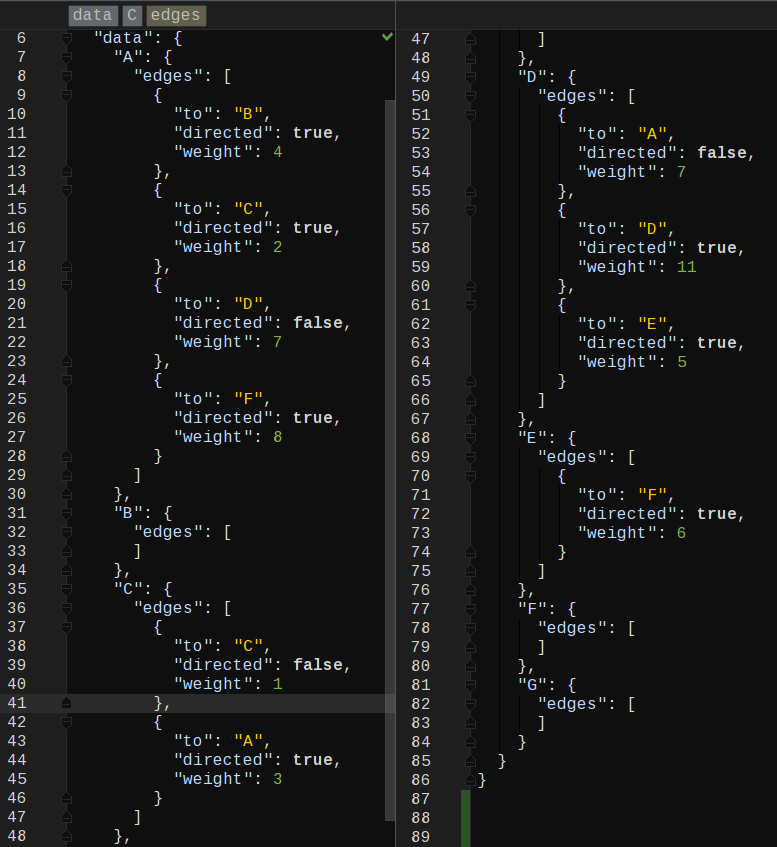
\includegraphics[width=1.2\textwidth]{figures/search_graph_json}
			\caption{Sample graph in the Graphinius JSON format}
			\label{fig:json_input_graph}
			\small Apart from the 'to' node, direction and weight, any node can exhibit an arbitrarily large feature vector containing any type of information (like patient data, word vectors, etc.). Another special sub-object which the input reader is looking for is the 'coords' object, which specifies the coordinates used in the constant layout renderer of the GraphiniusVIS library.
		\end{figure}
		
	
	\subsection{Graph Core}
	\label{ssect:graph_core}
	
		\subsubsection{Edges}
		\label{sssection: core_edges}
		
		\subsubsection{Nodes}
		\label{sssection: core_nodes}
		
		\subsubsection{Graph}
		\label{sssection: core_graph}
		
		\subsubsection{Traversal}
		\label{sssection: core_traveral}
		
		BFS / DFS implementations... [figure: callback-based DFS]
		
		\subsubsection{Degrees}
		\label{sssection: core_degrees}
		
		\subsubsection{Centralities}
		\label{sssection: core_centralities}
		
		\subsubsection{Generators}
		\label{sssection: core_}
		
	
	\subsection{Algorithms}
	\label{ssect:algorithms}
	
		\subsubsection{Clustering}
		\label{sssection: algo_clustering}
		
		\subsubsection{MinSpanTrees}
		\label{sssection: algo_minspan}
		
		\subsubsection{Shortest Paths}
		\label{sssection: algo_shorest_paths}


\section{The Op-Log}
\label{sect:op_log}

	\subsection{Timeline}
	\label{ssect:timeline}
	
	\subsection{History Object}
	\label{ssect:history_object}

	\subsection{Vocabulary}
	\label{ssect:vocabulary}	

	\subsection{Rendering Mechanism}
	\label{ssect:rendering}


\section{Graphinius VIS}
\label{sect:graphinius_vis}

	\subsection{2D/3D Mode}
	\label{ssect:vis_2d3d}
	
	\subsection{Navigation}
	\label{ssect:vis_navigation}
	
	\subsection{Graph Layouts}
	\label{ssect:vis_layouts}	
	
	\subsection{Interaction / Manipulation}
	\label{ssect:vis_interact_manipulate}
	
	\subsection{Timeline rewind / repeat}
	\label{ssect:vis_timeline}


\begin{landscape}
\begin{figure}[ht]
	\label{fig_history_workflow}
	\centering
	\vspace{-2.0cm}
%	\hspace*{0cm}
	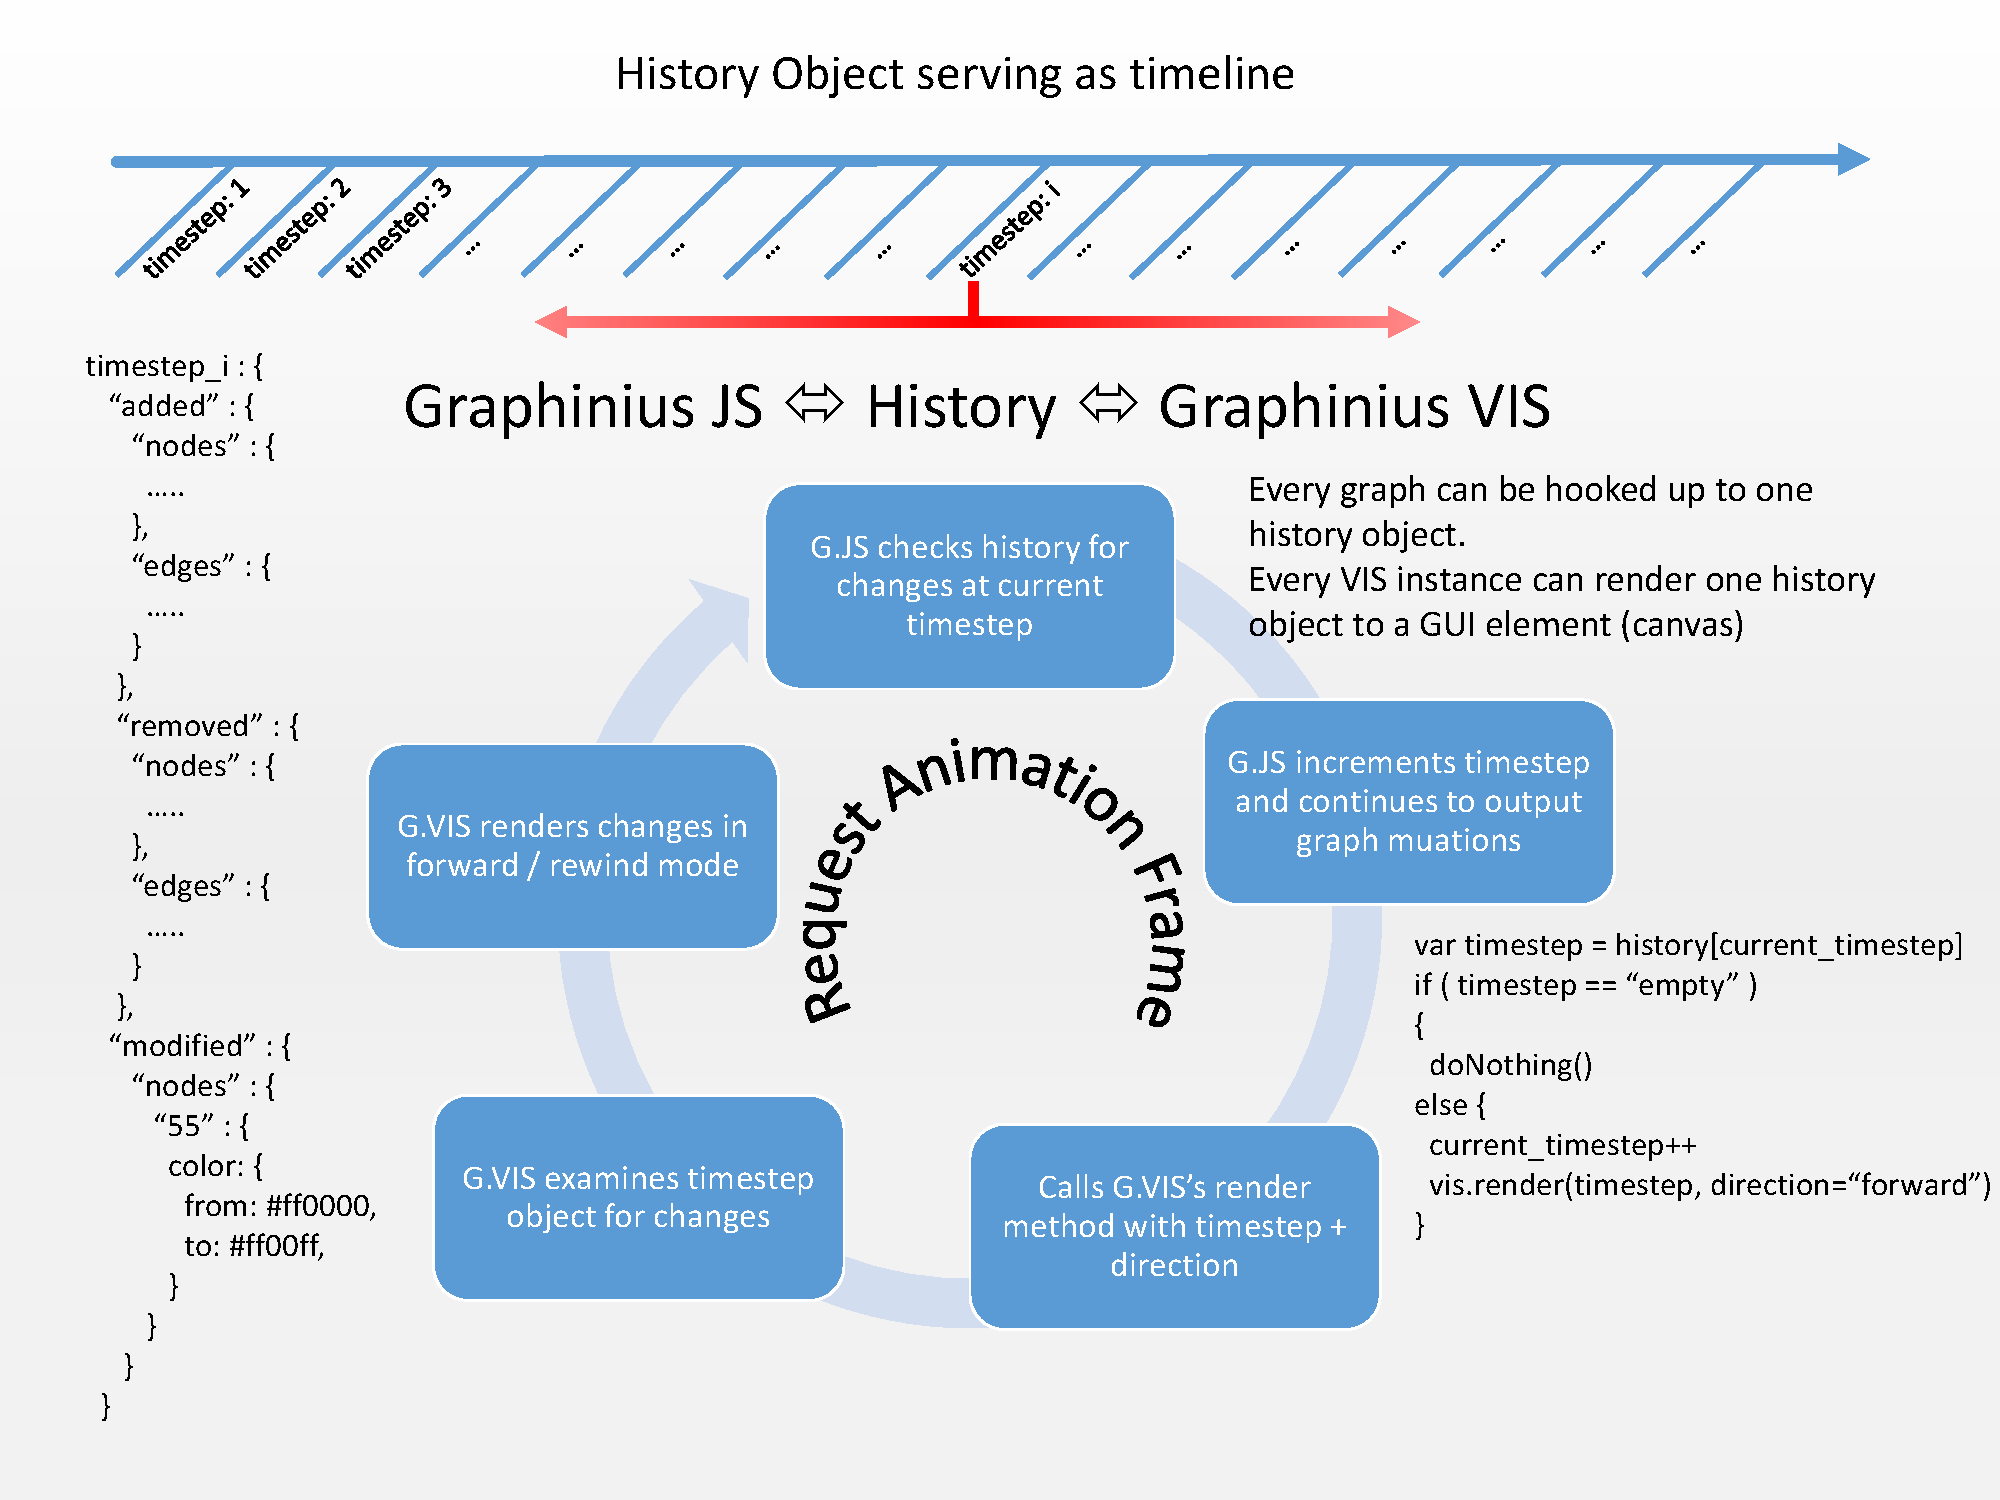
\includegraphics[width=1.6\textwidth]{figures/History_Workflow_pdf}
	\caption{Graphinius JS <-> VIS communication via Op-Log}
\end{figure}
\end{landscape}


\section{Areas of Applications (AoA)}
\label{sect:areas_of_applications}

	\subsection{Online Editor}
	\label{ssect:aoa_editor}
	
	\subsection{Biomedical Applications}
	\label{ssect:aoa_bioapps}
	
	\subsection{SN Anonymization}
	\label{ssect:aoa_anonym}


\section{Platform Services}
\label{sect:platform_services}

	\subsection{Personal Profile}
	\label{ssect:service_profile}
	
	\subsection{Teams}
	\label{ssect:service_teams}
	
	\subsection{Output / Reports}
	\label{ssect:service_output}